\documentclass[14pt]{extbook}
\usepackage{multicol, enumerate, enumitem, hyperref, color, soul, setspace, parskip, fancyhdr} %General Packages
\usepackage{amssymb, amsthm, amsmath, latexsym, units, mathtools} %Math Packages
\everymath{\displaystyle} %All math in Display Style
% Packages with additional options
\usepackage[headsep=0.5cm,headheight=12pt, left=1 in,right= 1 in,top= 1 in,bottom= 1 in]{geometry}
\usepackage[usenames,dvipsnames]{xcolor}
\usepackage{dashrule}  % Package to use the command below to create lines between items
\newcommand{\litem}[1]{\item#1\hspace*{-1cm}\rule{\textwidth}{0.4pt}}
\pagestyle{fancy}
\lhead{Makeup Progress Quiz 2}
\chead{}
\rhead{Version C}
\lfoot{2790-1423}
\cfoot{}
\rfoot{Summer C 2021}
\begin{document}

\begin{enumerate}
\litem{
Solve the linear equation below. Then, choose the interval that contains the solution.\[ \frac{4x + 3}{4} - \frac{4x -7}{3} = \frac{6x -7}{6} \]\begin{enumerate}[label=\Alph*.]
\item \( x \in [-0.78, -0.3] \)
\item \( x \in [3.1, 3.85] \)
\item \( x \in [12.36, 13.67] \)
\item \( x \in [0, 1.28] \)
\item \( \text{There are no real solutions.} \)

\end{enumerate} }
\litem{
Find the equation of the line described below. Write the linear equation in the form $ y=mx+b $ and choose the intervals that contain $m$ and $b$.\[ \text{Perpendicular to } 9 x + 7 y = 7 \text{ and passing through the point } (-8, -5). \]\begin{enumerate}[label=\Alph*.]
\item \( m \in [0.39, 1.13] \hspace*{3mm} b \in [-1.5, 0.4] \)
\item \( m \in [-1.48, -0.33] \hspace*{3mm} b \in [-14.6, -10.5] \)
\item \( m \in [0.39, 1.13] \hspace*{3mm} b \in [0.3, 2] \)
\item \( m \in [0.39, 1.13] \hspace*{3mm} b \in [2.4, 3.9] \)
\item \( m \in [0.87, 1.62] \hspace*{3mm} b \in [0.3, 2] \)

\end{enumerate} }
\litem{
Write the equation of the line in the graph below in Standard Form $Ax+By=C$. Then, choose the intervals that contain $A, B, \text{ and } C$.
\begin{center}
    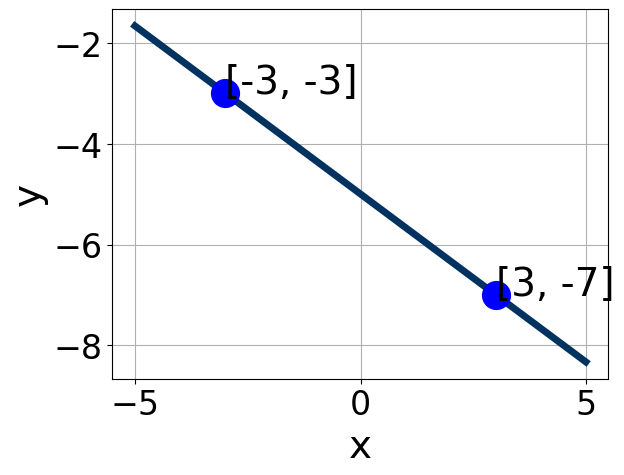
\includegraphics[width=0.5\textwidth]{../Figures/linearGraphToStandardCopyC.png}
\end{center}
\begin{enumerate}[label=\Alph*.]
\item \( A \in [0.4, 0.9], \hspace{3mm} B \in [-1.1, -0.84], \text{ and } \hspace{3mm} C \in [5, 6] \)
\item \( A \in [0.8, 2.4], \hspace{3mm} B \in [-3.16, -2.12], \text{ and } \hspace{3mm} C \in [9, 17] \)
\item \( A \in [0.8, 2.4], \hspace{3mm} B \in [1.85, 3.9], \text{ and } \hspace{3mm} C \in [-17, -8] \)
\item \( A \in [-2.2, -1.2], \hspace{3mm} B \in [-3.16, -2.12], \text{ and } \hspace{3mm} C \in [9, 17] \)
\item \( A \in [0.4, 0.9], \hspace{3mm} B \in [-0.47, 1.93], \text{ and } \hspace{3mm} C \in [-8, 1] \)

\end{enumerate} }
\litem{
First, find the equation of the line containing the two points below. Then, write the equation in the form $ y=mx+b $ and choose the intervals that contain $m$ and $b$.\[ (-2, -5) \text{ and } (6, 9) \]\begin{enumerate}[label=\Alph*.]
\item \( m \in [0.75, 3.75] \hspace*{3mm} b \in [-0.24, 1.69] \)
\item \( m \in [0.75, 3.75] \hspace*{3mm} b \in [-3.9, -2.15] \)
\item \( m \in [-7.75, -0.75] \hspace*{3mm} b \in [19.05, 20.67] \)
\item \( m \in [0.75, 3.75] \hspace*{3mm} b \in [2.13, 4.37] \)
\item \( m \in [0.75, 3.75] \hspace*{3mm} b \in [-1.63, -0.94] \)

\end{enumerate} }
\litem{
Solve the equation below. Then, choose the interval that contains the solution.\[ -2(-13x -11) = -14(-5x -18) \]\begin{enumerate}[label=\Alph*.]
\item \( x \in [-6, -4.9] \)
\item \( x \in [-4, -2.6] \)
\item \( x \in [-8, -6] \)
\item \( x \in [6, 6.9] \)
\item \( \text{There are no real solutions.} \)

\end{enumerate} }
\litem{
First, find the equation of the line containing the two points below. Then, write the equation in the form $ y=mx+b $ and choose the intervals that contain $m$ and $b$.\[ (7, -9) \text{ and } (-7, -11) \]\begin{enumerate}[label=\Alph*.]
\item \( m \in [-1.06, -0.12] \hspace*{3mm} b \in [-14, -10.2] \)
\item \( m \in [0.11, 0.46] \hspace*{3mm} b \in [8.9, 10.1] \)
\item \( m \in [0.11, 0.46] \hspace*{3mm} b \in [-10.3, -8.9] \)
\item \( m \in [0.11, 0.46] \hspace*{3mm} b \in [-16.5, -15.2] \)
\item \( m \in [0.11, 0.46] \hspace*{3mm} b \in [-6, -3.8] \)

\end{enumerate} }
\litem{
Solve the linear equation below. Then, choose the interval that contains the solution.\[ \frac{5x + 6}{7} - \frac{6x + 9}{4} = \frac{-9x + 9}{8} \]\begin{enumerate}[label=\Alph*.]
\item \( x \in [32.37, 36.37] \)
\item \( x \in [-0.69, 2.31] \)
\item \( x \in [-7.84, -4.84] \)
\item \( x \in [6.42, 9.42] \)
\item \( \text{There are no real solutions.} \)

\end{enumerate} }
\litem{
Find the equation of the line described below. Write the linear equation in the form $ y=mx+b $ and choose the intervals that contain $m$ and $b$.\[ \text{Parallel to } 3 x + 7 y = 10 \text{ and passing through the point } (-2, 4). \]\begin{enumerate}[label=\Alph*.]
\item \( m \in [-0.55, -0.28] \hspace*{3mm} b \in [5.6, 6.9] \)
\item \( m \in [0.05, 0.95] \hspace*{3mm} b \in [4, 5.3] \)
\item \( m \in [-0.55, -0.28] \hspace*{3mm} b \in [-3.3, -1.6] \)
\item \( m \in [-0.55, -0.28] \hspace*{3mm} b \in [1.3, 4.7] \)
\item \( m \in [-2.72, -2.15] \hspace*{3mm} b \in [1.3, 4.7] \)

\end{enumerate} }
\litem{
Write the equation of the line in the graph below in Standard Form $Ax+By=C$. Then, choose the intervals that contain $A, B, \text{ and } C$.
\begin{center}
    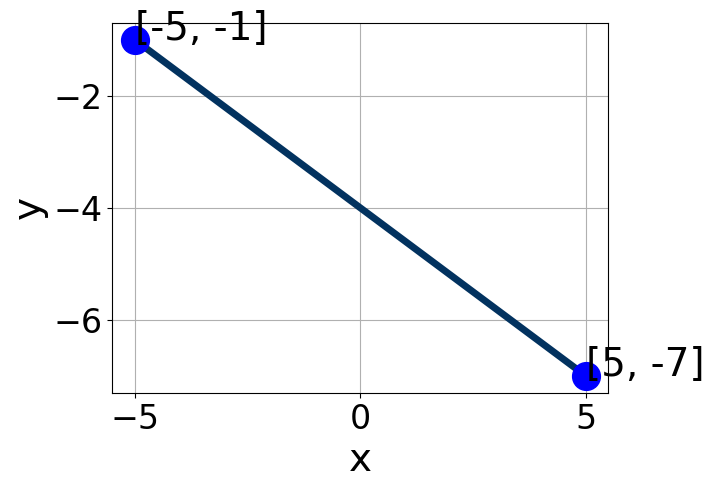
\includegraphics[width=0.5\textwidth]{../Figures/linearGraphToStandardC.png}
\end{center}
\begin{enumerate}[label=\Alph*.]
\item \( A \in [-3.54, -2.69], \hspace{3mm} B \in [-5.8, -2.9], \text{ and } \hspace{3mm} C \in [18, 23] \)
\item \( A \in [2.92, 3.89], \hspace{3mm} B \in [-5.8, -2.9], \text{ and } \hspace{3mm} C \in [18, 23] \)
\item \( A \in [0.48, 1.46], \hspace{3mm} B \in [-3.5, -0.2], \text{ and } \hspace{3mm} C \in [2, 5] \)
\item \( A \in [0.48, 1.46], \hspace{3mm} B \in [-0.1, 4.1], \text{ and } \hspace{3mm} C \in [-4, -2] \)
\item \( A \in [2.92, 3.89], \hspace{3mm} B \in [2.4, 6.8], \text{ and } \hspace{3mm} C \in [-20, -15] \)

\end{enumerate} }
\litem{
Solve the equation below. Then, choose the interval that contains the solution.\[ -19(6x -13) = -17(8x -18) \]\begin{enumerate}[label=\Alph*.]
\item \( x \in [25.07, 25.17] \)
\item \( x \in [-25.73, -24.72] \)
\item \( x \in [2.45, 2.86] \)
\item \( x \in [1.77, 2.63] \)
\item \( \text{There are no real solutions.} \)

\end{enumerate} }
\end{enumerate}

\end{document}